\documentclass{beamer} % blue; brown; gray; red;
%\documentclass[handout]{beamer}
%\usepackage{pgfpages}
%\usepackage{handoutWithNotes}
%\pgfpagesuselayout{4 on 1 with notes}[a4paper,border shrink=5mm]
%\pgfpagesuselayout{4 on 1}[a4paper,border shrink=5mm]
\usepackage{beamerthemesplit}
\usepackage{beamerthemeshadow}
%\usepackage[draft]{animate}
\usepackage{animate}
\usepackage{movie15}
\usepackage{graphics}
\usepackage{colortbl}
\usepackage{pgf,pgfarrows,pgfnodes,pgfautomata,pgfheaps}
\usepackage{amsmath,amssymb}
\usepackage{pgfpages}
\usepackage{tikz,pgffor}
\usetikzlibrary{shadows}
\usetikzlibrary{arrows}
\usetikzlibrary{calc,intersections,through,backgrounds}
\usepackage{ifthen}
\usetikzlibrary{shapes}
%%%%%%%%%%%%%%%%%%%%%%%%%%%%%%%%%%%%%%%%%%%%%%%%%%%%%%
\usepackage{xeCJK}
\usepackage{fontspec}
\setCJKmainfont[BoldFont=simhei.ttf]{simkai.ttf}
%\setCJKsansfont{simhei.ttf}
%\setCJKmonofont{simfang.ttf}
%%%%%%%%%%%%%%%%%%%%%%%%%%%%%%%%%%%%%%%%%%%%%%%%%%%%%%

%\setbeameroption{show notes}
%\setbeameroption{show only notes}
%\setbeameroption{show notes on second screen=right}



\usetheme{Warsaw}
%别的主题:Bergen,Boadilla,Madrid,AnnArbor,CambridgeUS,Pittsburgh, Rochester.
%有导航栏:Antibes,JuanLesPins,Montpellier,
%有内容的:Berkeley,PaloAlto,% Goettingen,Marburg,Hannover
%小导航栏:Berlin,Ilmenau,Dresden,Darmstadt, Frankfurt,Singapore,Szeged,
%章节表单:Copenhagen,Luebeck,Malmoe,Warsaw
\beamertemplateshadingbackground{red!10}{structure!10}
\beamertemplatesolidbackgroundcolor{white!90!blue}
\beamertemplatetransparentcovereddynamic
\beamertemplateballitem
\beamertemplatenumberedballsectiontoc
%\beamertemplatelargetitlepage
\beamertemplateboldpartpage

\usecolortheme{sidebartab}
%beetle,crane,dove,fly,seagull,wolverine,beaver
\renewcommand{\raggedright}{\leftskip=0pt \rightskip=0pt plus 0cm}
\raggedright
%%%%%%%%%%%%%%%%%%%%%%%%%%%%%%%%%%%%%%%%%%%%%%%%%%%%%%%%%%%%%%%%%%%%%%%%%%
\graphicspath{{figures/}}

\setbeamertemplate{caption}[numbered]
\newcommand{\animatepath}{./animate}
%%%%%%%%%%%%%%%%%%%%%%%%%%%%%%%%%%%%%%%%%%%%%%%%%%%%%%%%%%%%%%%%%%%%%%%%%%
\definecolor{MyDarkGreen}{rgb}{0.0,0.4,0.0}

\begin{document}
\renewcommand\contentsname{\bf 目录}
\renewcommand\figurename{\bf 图}
\renewcommand\tablename{\bf 表}
\renewcommand\refname{参考文献}


%%%%%%%%%%%%%%%%%%%%%%%%%%%%%%%%%%%%%%%%%%%%%%%%%%%%%%%%%%%%%%%%%%%%%%%%%%
\makeatletter
\usefoottemplate{ %重新定义页脚,加入作者,单位,单位图标,和文档标题
  \vbox{\tiny%
    \hbox{%
      \setbox\beamer@linebox=\hbox to\paperwidth{%
        \hbox to.5\paperwidth{
            \hfill\tiny\color{white}
                  \textbf{\insertshortauthor\quad\insertshortinstitute}
            \hskip .1cm\lower 0.2em\hbox{
\includegraphics[height=0.25cm]{./figures/CAS.pdf}}
            \hskip.3cm}%
        \hbox to.5\paperwidth{
            \hskip.3cm\tiny\color{white}
                  \textbf{\insertshorttitle}\hfill}\hfill}%
      \ht\beamer@linebox=2.625ex%
      \dp\beamer@linebox=0pt%
      \setbox\beamer@linebox=\vbox{\box\beamer@linebox\vskip1.125ex}%
      \color{structure}\hskip-\Gm@lmargin\vrule width.5\paperwidth
      height\ht\beamer@linebox\color{structure!70}\vrule width.5\paperwidth
      height\ht\beamer@linebox\hskip-\paperwidth%
      \hbox{\box\beamer@linebox\hfill}\hfill\hskip-\Gm@rmargin}
  }
}
\makeatother
%%%%%%%%%%%%%%%%%%%%%%%%%%%%%%%%%%%%%%%%%%%%%%%%%%%%%%%%%%%%%%%%%%%%%%%%%%
\title{复杂流体多尺度模拟方法与数值仿真研究}
\subtitle{力学研究所2014年(春季)硕博连读生转博答辩}
\institute[流固耦合系统力学重点实验室]{流固耦合系统力学重点实验室}
\author{周吕文 (导师:刘谋斌)}
\date{2013年11月7日}

%\pgfdeclaremask{zhou}{./Logo/CAS.pdf}
%\pgfdeclareimage[mask=zhou,height=2.5cm]{zhou}{./Logo/CAS.pdf}
%\titlegraphic{\pgfuseimage{zhou}}
%%%%%%%%%%%%%%%%%%%%%%%%%%%%%%%%%%%%%%%%%%%%%%%%%%%%%%%%%%%%%%%%%%%%%%%%%%
\frame[plain]{
\titlepage
\note{\textcolor{red}{[0-10s]}}
\note[item]{各位老师, 大家下午好}
\note[item]{我是流固耦合系统力学实验室周吕文, 我的导师是刘谋斌老师}
\note[item]{今天我答辩的题目是复杂流体多尺度模拟方法与数值仿真研究}
} 
\titlegraphic{\pgfuseimage{title}}
\AtBeginSection[]{ % 在每个Section前都会加入的Frame
  \frame<handout:0>{
    \frametitle{提纲}
    \tableofcontents[current,currentsubsection]
  }
}
\frame[Outline]{\frametitle{提纲}\tableofcontents
\note{\textcolor{red}{[10-15s]}}
\note[item]{答辩内容分为研究背景, 研究方法, 已做工作和研究计划四部分}
}
%%%%%%%%%%%%%%%%%%%%%%%%%%%%%%%%%%%%%%%%%%%%%%%%%%%%%%%%%%%%%%%%%%%%%%%%%%

\section{研究背景}
\subsection{问题背景}
\begin{frame}
\frametitle{问题背景}
\begin{columns}
\begin{column}[b]{0.35\textwidth}
\begin{center}
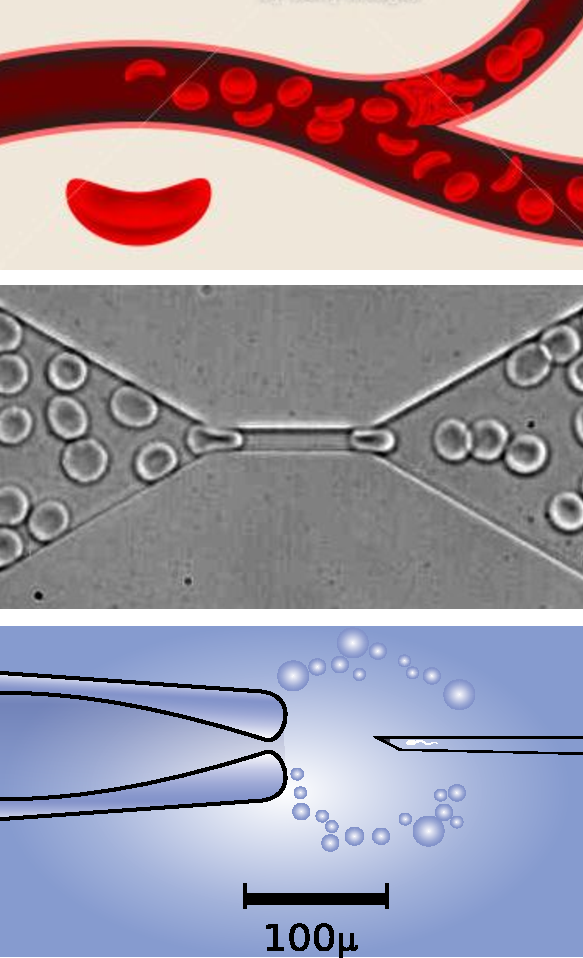
\includegraphics[width=0.9\textwidth]{microdivice.pdf}
\end{center}
\end{column}
\begin{column}[b]{0.65\textwidth}
复杂流体往往涉及多元, 多相, 多组分, 一般难以用牛顿流体模型描述. 复杂流体多尺度流动现象普遍存在于生命科学, 环境工程, 生化工程和微纳米科技等不同领域.\note{\textcolor{red}{[15-45s]}复杂流体的多尺度流动普遍存在于生命科学, 环境工程等不同领域.}
\begin{itemize}
\item 生物体内的体液流动, 包括毛细血管内的血液流动, 关系到生物体的健康. 
     \note[item]{比如毛细血管内的血液流动}
\item 生物微流动器件利用细胞的力学差异对正常细胞与病变细胞进行区分.
     \note[item]{微吸管法利用微流动判断和区分细胞是否病变}
\item 微针利用微流动可以高效而精确的对细胞, 局部组织等进行微小剂量的药物或高分子的输送. 
     \note[item]{微针利用微流动进行的卵胞浆内单精子注射.}
\end{itemize}
\end{column}
\end{columns}
\end{frame}

\subsection{研究现状}
\begin{frame}
\frametitle{不同尺度的方法}
\begin{figure}
\includegraphics<1>[width=\textwidth]{spatiotemporal.pdf}
\includegraphics<2>[width=\textwidth]{spatiotemporal1.pdf}
\includegraphics<3>[width=\textwidth]{spatiotemporal2.pdf}
\includegraphics<4>[width=\textwidth]{spatiotemporal3.pdf}
\note{\textcolor{red}{[45-100s]}对于不同尺度的问题,需要相应尺度的方法.}
\note<2->[item]{对于微观尺度的问题, 可以用分子动力学, 甚至量子计算来模拟. 分子动力学由于计算尺度的限制, 很难对介观尺度以上的流动进行模拟.}
\note<3->[item]{对于宏观问题, 可以用基于连续介质假设的NS方程来模拟. 当问题所涉及的空间尺度逐渐缩小到介观乃至微观时, NS方程就未必适用.}
\note<4->[item]{对于介于微观和宏观尺度, 我们称为介观, 常用的介观尺度的方法有耗散粒子动力学, 布勆动力学等方法. 布朗动力学等不大适合模拟处理含生物高分子, 细胞等的复杂流体行为. 最终我们选择了耗散粒子动力学方法.}
\end{figure}
\end{frame}

%\begin{frame}
%\frametitle{常用方法的不足}
%复杂流体的多尺度计算模型涉及从微观到介观甚至宏观尺度的时间和空间流体动力学特征.
%\note{\textcolor{red}{[100-130s]}我们研究的对象主要是介观尺度流动现象, 直接相关的物理特性往往处于毫秒, 微米级, 因此介于纳米与毫米之间的介观尺度模拟方法合理选择.}
%\begin{itemize}
%\item 传统的网格方法一般基于连续介质力学假设, 当问题所涉及的空间尺度逐渐缩小到介观乃至微观时未必适用. 
%     \note[item]{传统的网格方法一般基于连续介质力学假设, 对于介观乃至微观的问题未必适用.}
%\item 由于当前计算条件的限制,分子动力学模拟所涉及的时间及空间尺度还仅限于纳秒和纳米级,很难对介观尺度以上的流动区域进行模拟. 
%     \note[item]{而分子动力学方向又因为计算尺度的限制, 很难对介观尺度以上的流动进行模拟.}
%\item 作为介观尺度的方法, 布朗动力学, 格子气自动机及网格波尔兹曼等不大适合模拟处理含生物高分子, 细胞等的复杂流体行为.
%     \note[item]{作为观尺度的方法, 布朗动力学, 格子气自动机等不大适合模拟处理含生物高分子, 细胞等的复杂流体行为.}
%\end{itemize}
%\end{frame}

\section{研究方法}
\subsection{耗散粒子动力学}
\frame{ \frametitle{耗散粒子动力学简介}
\note{\textcolor{red}{[100-130s]}下面简要介绍一下耗散粒子动力学:}
  \begin{itemize}
  \item 耗散粒子动力学(DPD)是一种粗粒化的分子动力学方法,适合模拟介观尺度的简单和复杂流体动力学和流变性能.
        \note[item]{耗散粒子动力学(DPD)是一种粗粒化的分子动力学方法}
  \item 由Hoogerbrugge与Koelman首先提出, 旨在解决经典分子动力学难以解决的流体
        时间和空间尺度问题.
        \note[item]{提出这一方法的目的是为了解决经典分子动力学难以解决的流体时间和空间尺度问题}
  \item 优点: 与经典分子动力学方法相比, DPD方法可以使用更大的粒子尺寸和更长的时间步长, 因此具有更好的计算效率与计算能力,能应用到介观尺度乃至亚宏观的问题.
        \note[item]{因此相对于经典分子动力学, DPD由于可以使用更大的粒子尺寸和更长的时间步长,而且有更好的计算效率与计算能力.}
  \item 应用: 各类复杂的流体流动, 如相分离, 蛋白质等大分子悬浮, 表面活性剂, 胶
        体输运, 稀释聚合物溶液, 生物薄膜, 以及介观尺度的多相流动现象.
        \note[item]{现在的应用也相当广泛.}
  \end{itemize}
}

\frame{\frametitle{运动方程}
\begin{columns}
\begin{column}[c]{0.35\textwidth}
\begin{center}
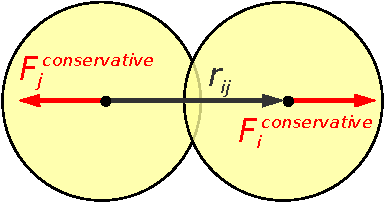
\includegraphics[width=0.9\textwidth]{conservative.pdf}
\vspace{1em}

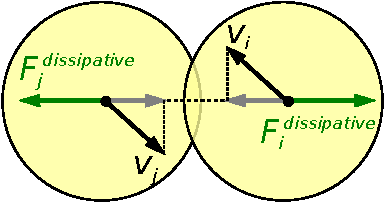
\includegraphics[width=0.9\textwidth]{dissipative.pdf}
\vspace{1em}

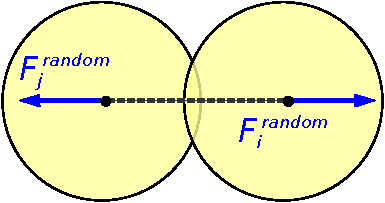
\includegraphics[width=0.9\textwidth]{random.pdf}
\end{center}
\end{column}
\begin{column}[c]{0.65\textwidth}
\note{\textcolor{red}{[130-145s]}}
牛顿运动方程描述DPD粒子运动\note[item]{DPD模型中粒子的运动由牛顿运动方程描述.}
  \[
  \frac{d\mathbf{r}_i}{dt} = \mathbf{v}_i,   
  \frac{d\mathbf{v}_i}{dt} = \mathbf{f}_i = \mathbf{f}_i^{\text{int}} + \mathbf{f}_i^{\text{ext}}
  \]
\note[item]{耗散粒子动力学中的粒子除了受到保守力外, 还受到耗散力和随机力.}
%\note[item]{耗散力方向与粒子间相对运动的方向相反, 因此通常会减弱粒子间相互作用, 减少系统的动能, 降低系统的温度.}
%\note[item]{而随机力则通常引起粒子间的随机振动, 增加系统的动能, 提高系统的温度.}
%\note[item]{耗散力和随机力的相互作用, 在满足一定条件下, 能使整个系统温度维持在基本恒定的水平上.}
DPD粒子间作用力包括保守力, 耗散力及随机力:
  \[
  \textcolor{red}{\mathbf{F}_{ij}^C = a_{ij}w^C(r_{ij})\mathbf{\hat{r}}_{ij}}
  \]
  \[
  \textcolor{MyDarkGreen}{\mathbf{F}_{ij}^D = -\gamma w^D(r_{ij})\Big(\mathbf{\hat{r}}_{ij}\cdot \mathbf{v}_{ij}\Big)\mathbf{\hat{r}}_{ij}}
  \]
  \[
  \textcolor{blue}{\mathbf{F}_{ij}^R = \sigma w^R(r_{ij})\xi_{ij}\mathbf{\hat{r}}_{ij}}
  \]
保守力权函数$w^C(r_{ij})$, 一般取为$1-r_{ij}$.
\end{column}
\end{columns}
}


\subsection{珠簧链模型}

\frame{\frametitle{珠簧链模型}
\begin{columns}
\begin{column}[c]{0.5\textwidth}
\begin{figure}
\centering
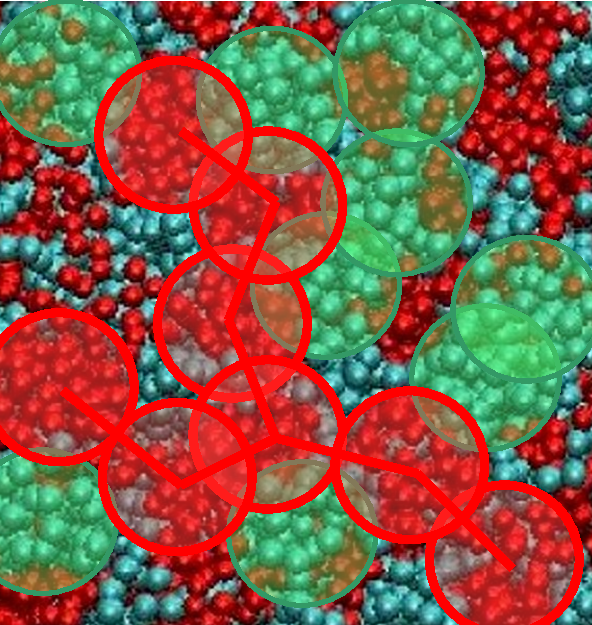
\includegraphics[width=\textwidth]{polymer.pdf}
\end{figure}
\end{column}
\begin{column}[c]{0.5\textwidth}
\note{\textcolor{red}{[145-165s]} 在DPD方法中, 模拟高分子时常用珠簧链模型, 把高分子链抽象成由弹簧力连接的DPD粒子. 下面是三种常用的珠簧链模型.}
\begin{itemize}
\item 简谐珠-簧链模型
\[
U_{\text{harmonic}} = \frac{k_s}{2}(l-l_0)^2
\]
\item FENE珠-簧链模型
\[
U_{\text{FENE}} = -\frac{k_s}{2}l_m^2\log(1-x^2)
\]
\item WLC珠-簧链模型
\[
U_{\text{WLC}} = \frac{k_B T l_m}{4p}\frac{3x^2-2x^3}{1-x}
\]
\end{itemize}
\end{column}
\end{columns}
}

\section{已做工作}
\subsection{研究思路}
\begin{frame}
\frametitle{研究思路}
\tikzstyle{decision} = [diamond,aspect=2, draw,fill=red!20, 
    text width=32, text badly centered, inner sep=0pt]

\tikzstyle{block} = [rectangle, draw=gray, gray,
    text width=43, text centered, rounded corners, minimum height=25]
\tikzstyle{selectblock} = [rectangle, draw=black, black, fill=blue!20,
    text width=43, text centered, rounded corners, minimum height=25]

\tikzstyle{line} = [draw,->, >=stealth',shorten >=1pt,auto,thick, gray]
\tikzstyle{selectedline} = [draw,->, >=stealth',shorten >=1pt,auto,thick]
\tikzstyle{selectededge} = [draw,line width=2pt,->,red!50,>=stealth',shorten >=-1pt,auto]
{\footnotesize
\begin{tikzpicture}[scale=0.76]
    \clip (-1.3,-5.75) rectangle (15,4.35);
    \coordinate (start)  at ( 0,  -1); % 研究内容
    \coordinate (app)    at ( 3,  -1); % 应用
    \coordinate (method) at ( 3, 3.5); % 方法
    \coordinate (mpi)    at ( 3,-4.5); % 并行 CPU/GPU
    \coordinate (couple) at ( 6, 3.5); % MD, DPD, SPH藕合
    \coordinate (DNA)    at ( 6, 0.0); % 高分子
    \coordinate (RBC)    at ( 6,-2.0); % 红细胞
    \coordinate (field)  at ( 6, 1.5); % 多物理场
    \coordinate (cell)   at ( 6,-3.5); % 乳腺癌细胞
    \coordinate (scale)  at (12,-1  ); % 高性能大规模计算
    \coordinate (poten)  at (3 ,1.5 ); % 势函数
    \coordinate (simple) at (3 ,-2.8);
    \coordinate (A)      at (3 ,0.25);
    \coordinate (spring) at (9.5,-1);

    \foreach  \name/             \lab/  \fill/     \color/ \start / \ended in {
              start/          研究内容/  blue!20/black!50 /1 /1 ,
                app/              应用/  blue!20/black!80/ 1 /2 ,
             method/              方法/  blue!20/black!80/ 1 /2 ,
                mpi/    {并行 CPU/GPU}/  blue!20/black!80/ 1 /2 ,
             couple/{MD, DPD, SPH藕合}/  blue!20/black!80/ 1 /3 ,
              poten/           势函数/   blue!20/black!80/ 1 /3 ,
                DNA/            高分子/  blue!20/black!80/ 1 /6 ,
                RBC/            红细胞/  blue!20/black!80/ 1 /9 ,
              field/          多物理场/  blue!20/black!80/ 1 /8 ,
               cell/        乳腺癌细胞/  blue!20/black!80/ 1 /10 ,
              scale/  高性能大规模计算/  blue!20/black!80/ 1 /12
                                                      }
        \node<\start-\ended>(\name)[block] at (\name) {\lab};


    \foreach \source/ \dest/\plot/ \start/ \ended in {
               start/method/|-/1/2,
               start/app/--/1/2,
               start/mpi/|-/1/2,
               method/couple/--/1/3,
               method/poten/--/1/3,
               app/RBC/-|/1/9,
               app/DNA/-|/1/6,
               RBC/cell/--/1/10,
               DNA/field/--/1/9,
               poten/app/--/1/4,
               couple/A/{--(6,2.5)--(4.5,2.5)--(4.5,0.25)--}/1/4,
               couple/{12.5,-0.4}/{--(12.5,3.5)--}/1/11,
               mpi/{12.5,-1.6}/{--(12.5,-4.5)--}/1/11,
               scale/field/|-/1/12,
               scale/DNA/|-/1/12,
               scale/RBC/|-/1/12,
               scale/cell/|-/1/12
}
       \path<\start-\ended> [line] (\source) \plot (\dest);


    \foreach  \name/             \lab/  \fill/     \color/ \start / \ended in {
              start/          研究内容/  blue!20/black!50 /2 / 14,
                app/              应用/  blue!20/black!80/ 3 / 14,
             method/              方法/  blue!20/black!80/ 3 / 14,
                mpi/    {并行 CPU/GPU}/  blue!20/black!80/ 3 / 14,
             couple/{MD, DPD, SPH藕合}/  blue!20/black!80/ 4 / 14,
              poten/           势函数/   blue!20/black!80/ 4 / 14,
                DNA/            高分子/  blue!20/black!80/ 7 / 14,
                RBC/            红细胞/  blue!20/black!80/ 10 / 14,
              field/          多物理场/  blue!20/black!80/ 9 / 14,
               cell/        乳腺癌细胞/  blue!20/black!80/11 / 14,
              scale/  高性能大规模计算/  blue!20/black!80/ 12 / 14
                                                      }
        \node<\start-\ended>(\name)[selectblock] at (\name) {\lab};


    \foreach \source/ \dest/\plot/ \start/ \ended in {
               start/method/|-/3/ ,
               start/app/--/3/ ,
               start/mpi/|-/3/ ,
               method/couple/--/4/,
               method/poten/--/4/,
               app/RBC/-|/10/ ,
               app/DNA/-|/7/ ,
               RBC/cell/--/11/,
               DNA/field/--/9/ ,
               poten/app/--/5/ ,
               couple/A/{--(6,2.5)--(4.5,2.5)--(4.5,0.25)--}/5/,
               couple/{12.5,-0.4}/{--(12.5,3.5)--}/12/,
               mpi/{12.5,-1.6}/{--(12.5,-4.5)--}/12/,
               scale/field/|-/13/ ,
               scale/DNA/|-/13/ ,
               scale/RBC/|-/13/ ,
               scale/cell/|-/13/
}
       \path<\start-\ended>[selectedline] (\source) \plot (\dest);

\node<1-5,7-> (simple) [decision, fill=none, draw=gray, gray] at (simple) {\scriptsize 简单流体};
\path<1-5,7-> [line] (simple)--node[left]{\tiny 验证} (app);
\node<6> (simple) [decision] at (simple) {\scriptsize 简单流体};
\path<6> [selectedline] (simple)--node[left]{\tiny 验证} (app);

\node<1-7,11-> (spring)[decision, fill=none, draw=gray, gray] at (spring) {\scriptsize 珠簧链};
\node<8-10> (spring) [decision] at (spring) {\scriptsize 珠簧链};

\path<1-7,9-> [line] (DNA)--node[sloped]{\tiny 验证} (spring);
\path<1-9,11->(spring) [line] (spring)--node[sloped]{\tiny 应用} (RBC);

\path<8> [selectedline] (DNA)--node[sloped]{\tiny 验证} (spring);
\path<10>[selectedline] (spring)--node[sloped]{\tiny 应用} (RBC);


\begin{pgfonlayer}{background}
        \foreach \source / \dest / \plot/ \start / \ended in {
               start/method/|-/3/3,
               start/app/--/3/3,
               start/mpi/|-/3/3,
               method/couple/--/4/4,
               method/poten/--/4/4,
               app/RBC/-|/10/10,
               app/DNA/-|/7/7,
               RBC/cell/--/11/11,
               DNA/field/--/9/9,
               poten/app/--/5/5,
               couple/A/{--(6,2.5)--(4.5,2.5)--(4.5,0.25)--}/5/5,
               couple/{12.5,-0.4}/{--(12.5,3.5)--}/12/12,
               mpi/{12.5,-1.6}/{--(12.5,-4.5)--}/12/12,
               scale/field/|-/13/13,
               scale/DNA/|-/13/13,
               scale/RBC/|-/13/13,
               scale/cell/|-/13/13
                                                      }{
            %\path<\fr-\en>[selected edge,-,line width=3pt,shorten >=3pt] (\source) -- (\dest);
            \path<\start-\ended>[selectededge] (\source) \plot (\dest);}


\path<6> [selectededge] (simple)-- (app);
\path<8> [selectededge] (DNA)-- (spring);
\path<10> [selectededge] (spring)-- (RBC);
\end{pgfonlayer}
\end{tikzpicture}}

\note{\textcolor{red}{165-250s}}
\note<3->[item]{研究内容主要分为方法, 应用和并行三大块.}
\note<4->[item]{对于方法, 主要是考虑改进DPD势函数和藕合MD,DPD,SPH方法.}
\note<5->[item]{方法上的工作最终要反馈给应用.}
\note<6->[item]{对于应用, 在做正式的工作前, 用简单流体的流动检验方法和程序.}
\note<7->[item]{在此基础上, 我们模拟并研究了高分子在微通道中运动与悬浮.}
\note<8->[item]{同时也验证了珠簧链模型的可行性.}
\note<9->[item]{下一步再把高分子的模拟推广到多物理场, 比如电场.}
\note<10->[item]{另一方面应用是在红细胞的运动与变形模拟方面, 我们利用珠簧链模型来构造红细胞膜.}
\note<11->[item]{在此基础上, 再把模型由红细胞推广到其它细胞, 比如我们现在选择的乳腺癌细胞.}
\note<12->[item]{对于并行, 结合藕合算法, 行成一套高性能大规模的程序}
\note<13->[item]{最后再把它反馈各个应用中, 做一些多尺度大规模拟计算, 由单个或数个红细胞的模拟发展成一段毛细血管内的血液流动的模拟}
%
\tikzstyle{decision} = [diamond,aspect=2, draw,fill=blue!20, 
    text width=32, text badly centered, inner sep=0pt]
\tikzstyle{block} = [rectangle, draw, fill=blue!20, 
    text width=43, text centered, rounded corners, minimum height=25]
\tikzstyle{line} = [draw, -latex', very thick]
\tikzstyle{cloud} = [draw, ellipse,fill=red!20, node distance=75,
    text width=28, minimum height=0]
{\footnotesize
\begin{tikzpicture}[scale=0.76]
    % Place nodes
    \node [block](A) at (0,-1) {\bf 研究内容};
    \node [block](B) at (3,-1) {\bf 应用};
    \node [block](C) at (3,3.5) {\bf 方法};
    \node [block](D) at (3,-4.5) {\bf 并行 CPU/GPU};

    \node [block](E) at (6,0.0) {高分子};
    \node [block](F) at (6,-2.0) {红细胞};
    \node [block, fill=red!30](G) at (6,3.5) {\textcolor{blue}{MD, DPD, SPH藕合}};
    %\node [block](H) at (6,-3.5) {CPU};

    \node [block, fill=red!30](I) at (6,1.5) {\textcolor{blue}{多物理场}};
    \node [block, fill=blue!20](J) at (6,-3.5) {\textcolor{blue}{乳腺癌细胞}};
    %\node [block](K) at (9,-3.5) {\textcolor{blue}{GPU}};

    \node [block, fill=red!30](L) at (12,-1) {\textcolor{blue}{高性能大规模计算}};

    \node [block, fill=red!30](M) at (3,1.5) {\textcolor{blue}{势函数}};
    \node [decision](N) at (9.5,-1) {\scriptsize 珠簧链};
    \node [decision](O) at (3,-2.8) {\scriptsize 简单流体};

    \path [line] (A) -- (B);
    \path [line] (A) |- (C);
    \path [line] (A) |- (D);
    \path [line] (B) -| (E);
    \path [line] (B) -| (F);
    \path [blue, line, dashed] (C) -- (G);

    \path [line] (E) -- (I);
    \path [line] (F) -- (J);

    \path [blue, line, dashed] (D) --(12.5,-4.5)-- (12.5,-1.6);
    \path [blue, line, dashed] (G) --(12.5,3.5)-- (12.5,-0.4);
    \path [blue, line, dashed] (G) -- (6,2.5) -- (4.5,2.5)-- (4.5, 0.25) -- (3, 0.25);
    \path [blue, line, dashed] (L) |- (I);
    \path [blue, line, dashed] (L) |- (J);
    \path [blue, line, dashed] (L) |- (E);
    \path [blue, line, dashed] (L) |- (F);

    \path [blue, line, dashed] (C) -- (M);
    \path [blue, line, dashed] (M) -- (B);
    
    \path [line] (E)--node[sloped, fill=red!8.5]{\tiny 验证} (N);
    \path [line] (N)--node[sloped, fill=red!8.5]{\tiny 应用} (F);
    \path [line] (O)--node[left]{\tiny 验证} (B);

\end{tikzpicture}}

\end{frame}

\subsection{高分子在微通道中运动与悬浮的DPD模拟}
\begin{frame}
\frametitle{简单流体及高分子溶液泊肃叶流的DPD模拟}
\note{\textcolor{red}{250-270s}}
\note[item]{下面具体介绍一下我目前已经做或正在做的工作. 第一方面的工作是高分子在微通道中运动与悬浮的DPD模拟}
\note[item]{首先我们在成功模拟简单流体的基础上, 模拟了高分子在简单直管道中的运动与迁移.}
\begin{columns}
\begin{column}[c]{0.5\textwidth}
\begin{figure}
\centering
\animategraphics[width=\textwidth, poster=first, autoplay, every = 2]{5}{./animate/Poise/}{1}{16}
\caption{简单流体的泊肃叶流}
\end{figure}
\end{column}
\begin{column}[c]{0.5\textwidth}
\begin{figure}
\centering
\animategraphics[width=\textwidth, poster=first, autoplay, every = 2]{5}{./animate/Chain=/}{1}{30}
\caption{高分子溶液的泊肃叶流}
\end{figure}
\end{column}
\end{columns}
\end{frame}

\begin{frame}
\frametitle{不同微通道中高分子运动与悬浮的DPD模拟}
\note{\textcolor{red}{270-280s}}
\note[item]{其次我们还对微缩通道中的高分子运动与悬浮进行了模拟.}
\begin{columns}
\begin{column}[c]{0.5\textwidth}
\begin{figure}
\centering
\animategraphics[width=\textwidth, poster=first, autoplay, every = 2]{5}{./animate/ChainT/}{1}{30}
\caption{方型微缩直通道}
\end{figure}
\end{column}
\begin{column}[c]{0.5\textwidth}
\begin{figure}
\centering
\animategraphics[width=\textwidth, poster=first, autoplay, every = 2]{5}{./animate/ChainY/}{1}{30}
\caption{坡型微缩通道}
\end{figure}
\end{column}
\end{columns}
\end{frame}


%\begin{frame}
%\frametitle{高分子溶液水平方向速度, 温度, 密度}
%\begin{columns}
%\begin{column}[c]{0.5\textwidth}
%\begin{figure}
%\centering
%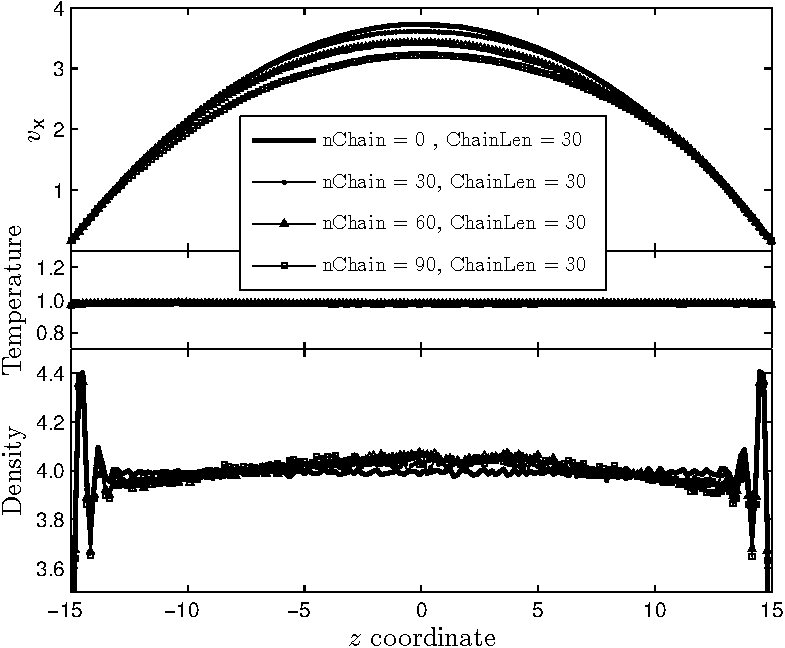
\includegraphics[width=\textwidth]{changChain1.pdf}
%\caption{微直道}
%\end{figure}
%\end{column}
%\begin{column}[c]{0.5\textwidth}
%\begin{figure}
%\centering
%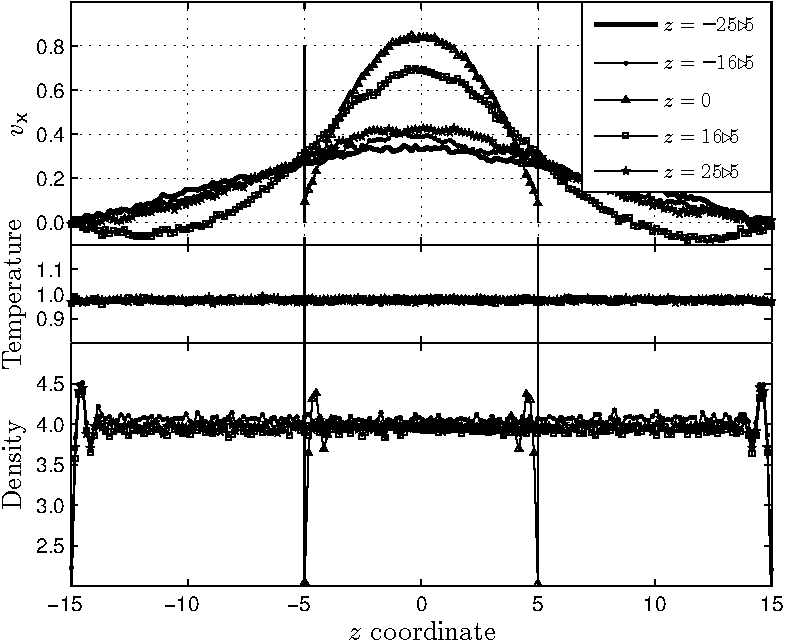
\includegraphics[width=\textwidth]{Tprof.pdf}
%\caption{方型微缩直通道}
%\end{figure}
%\end{column}
%\end{columns}
%\end{frame}


\begin{frame}
\frametitle{高分子在槽道中运动与悬浮的DPD模拟}
\note{\textcolor{red}{280-295s}}
\note[item]{最后我们把对高分子运动与悬浮的模拟推广到复杂的槽道中.}
\note[item]{图上显示的是部分高分子在不同时刻的构型图}
\begin{center}
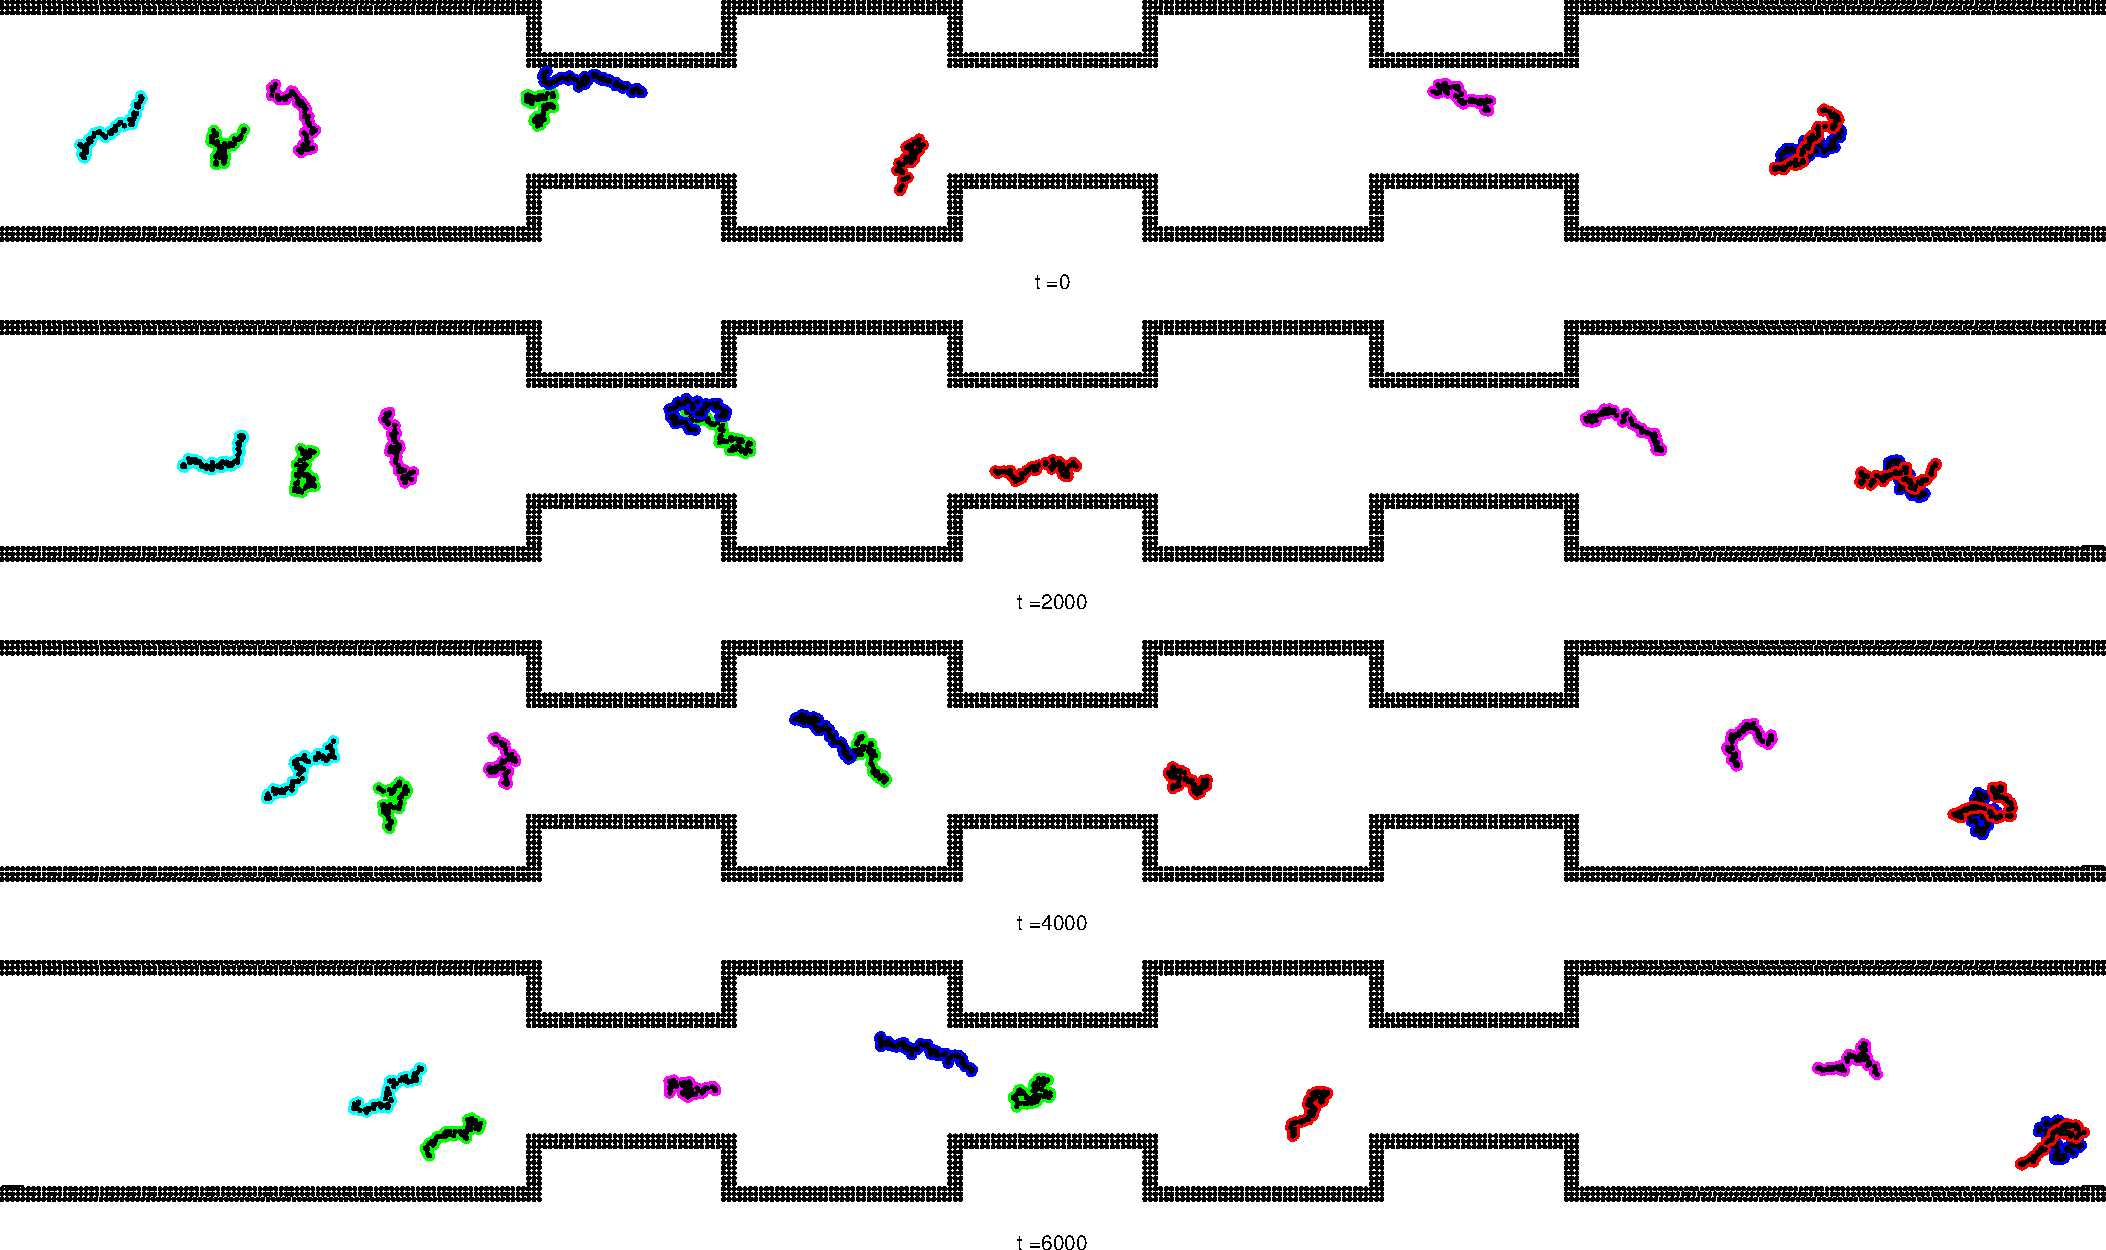
\includegraphics[width=\textwidth]{configchains.pdf}
\end{center}
\end{frame}

\begin{frame}
\frametitle{高分子在槽道中运动与悬浮的DPD模拟}
\note{\textcolor{red}{295-310s}}
\note[item]{我们还计算并比较了不同高分子长度和数量对流场的影响, 这里我们展示了部分物理场, 图5-图7分别为的水平速度场, 温度场, 密度场.}
\begin{figure}
\centering
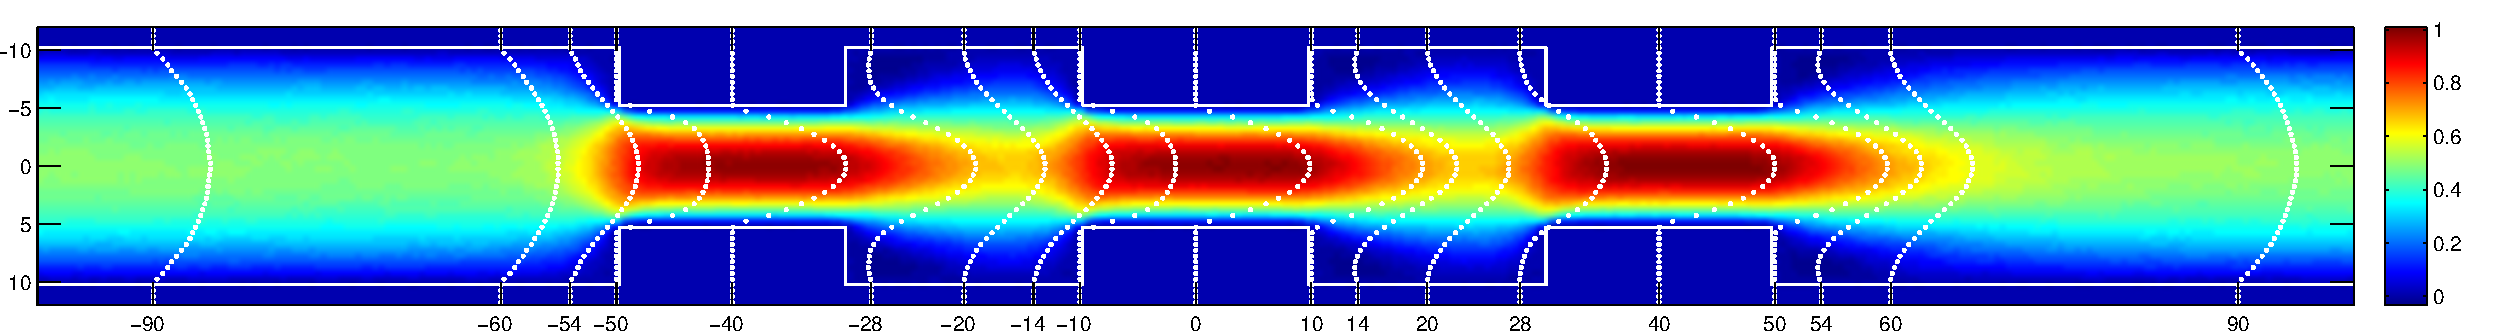
\includegraphics[width=\textwidth]{vxprofile.pdf}
\vspace{-2em}
\caption{水平速度场}
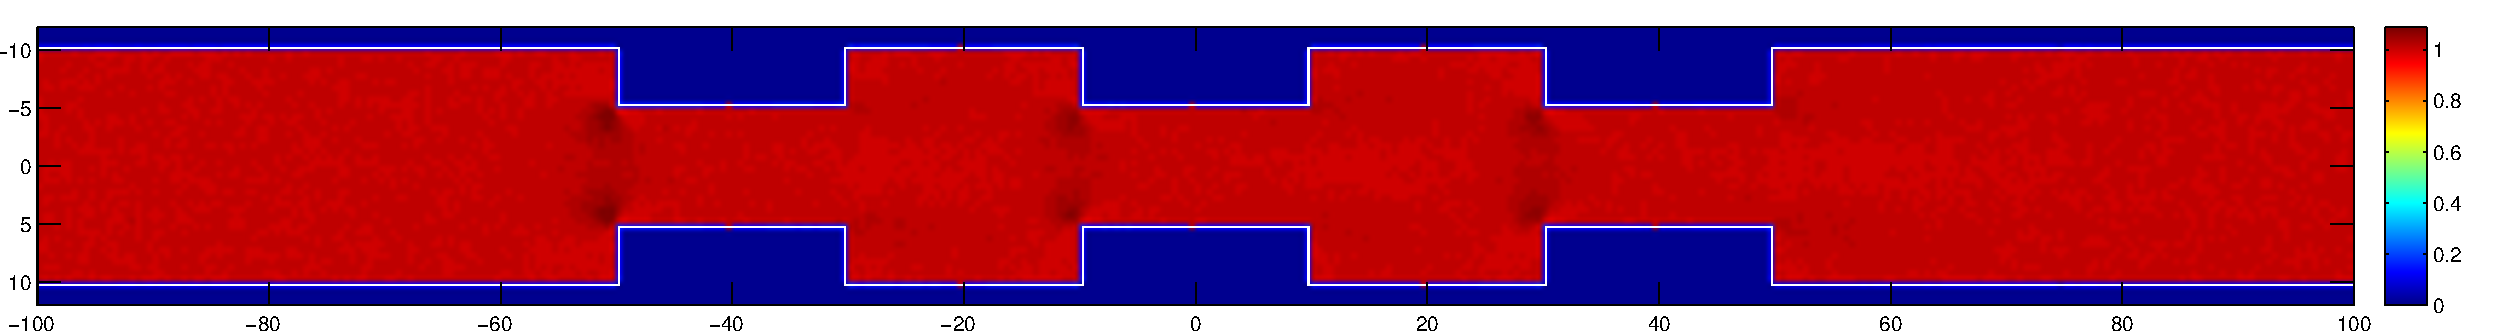
\includegraphics[width=\textwidth]{t.pdf}
\vspace{-2em}
\caption{温度场}
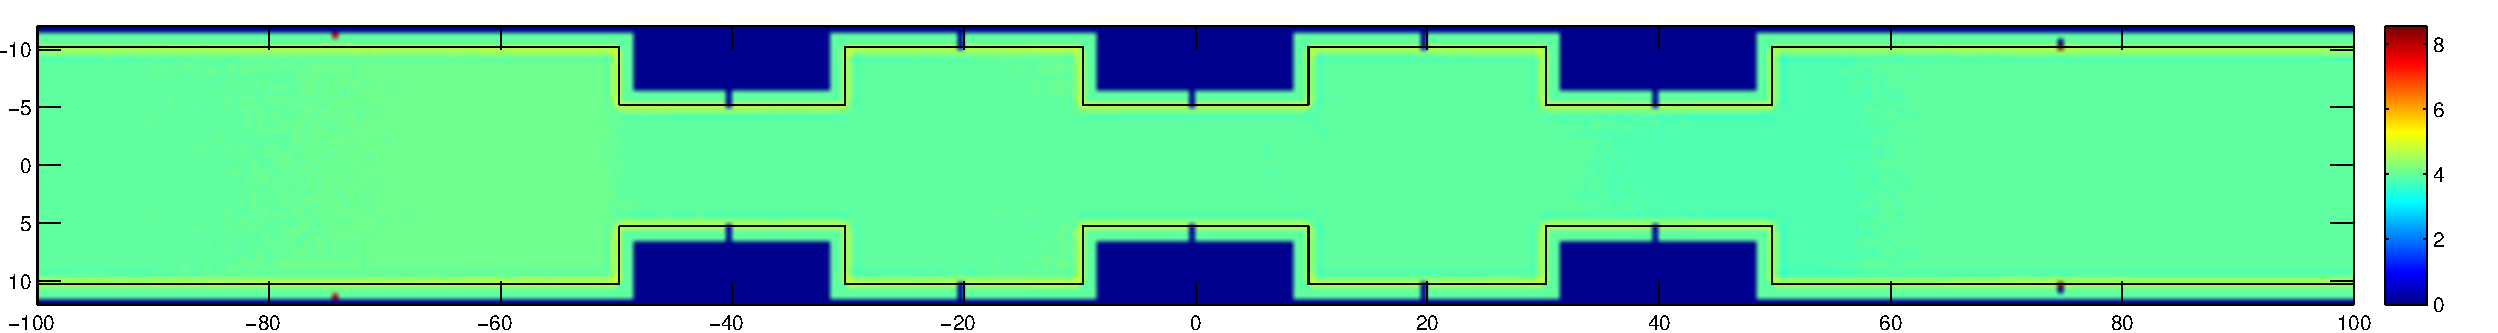
\includegraphics[width=\textwidth]{rho.pdf}
\vspace{-2em}
\caption{密度场}
\end{figure}
\end{frame}


\begin{frame}
\frametitle{高分子在微通道中运动与悬浮的DPD模拟: 小结}
\note{\textcolor{red}{310-330s}}
\note[item]{对于高分子运动与悬浮的模拟, 目前我们得到了一些有关高分子在运动中表现出来的行为,对流场的影响等方面定性和定量的结果和结论, 并发表了两篇期刊论文.}
\begin{itemize}
\item 高分子链对沿高度方向的水平速度及密度则有较明显影响. 高分子链的存在降低周围流体粒子的流动速度, 引起局部粒子密度波动, 形成比较明显的拖曳现象. 
\item 高分子链伸展程度: 通道边界区域 $>$ 通道中心区域; 
微直通道$>$斜坡微缩通道$>$方形微缩通道.
\item 微通道结构上细微的差别也会对系统的产生明显产生差异. % 主要体现在速度和密度
\item 高分子链会根据周围流动, 自动调整其构型, 以便更有利的快速顺利的通过微通道.
\end{itemize}

\textcolor{blue}{\scriptsize \bf Zhou L. V., Liu M. B.* and Chang, J. Z., \it{Acta Polymerica Sinica} 7: 720-727, 2012.} 

\textcolor{blue}{\scriptsize \bf Zhou L. V., Liu M. B.* and Chang J. Z., \it{Interaction and Multiscale Mechanics} 6(2): 157-172, 2013.}

\end{frame}



\subsection{血红细胞与癌细胞的DPD模拟}
\begin{frame}
\frametitle{红细胞的运动与变形模拟: 红细胞膜结构}
\note{\textcolor{red}{330-350s}}
\note[item]{另一方面, 我们还对红细胞的运动与变形进行了模拟}
\note[item]{图8是血红细胞的模结构, 红细胞膜主要由双分子层, 跨膜蛋白及膜下的血影蛋白网组成. 血影蛋白网是细胞的主要骨架}
\begin{figure}[!htb]
\centering
\begin{tikzpicture}[scale=0.7]
\foreach \xf/\yf/\xs/\ys in {
2.9900/5.0400/2.9900/5.0400,
 2.9900/5.0400/4.7900/5.1000,
 2.9900/5.0400/1.3800/3.3900,
 2.9900/5.0400/3.6300/3.7100,
 4.7900/5.1000/4.7900/5.1000,
 4.7900/5.1000/6.9100/5.1300,
 4.7900/5.1000/3.6300/3.7100,
 4.7900/5.1000/5.7100/3.7300,
 6.9100/5.1300/6.9100/5.1300,
 6.9100/5.1300/8.6400/5.0900,
 6.9100/5.1300/5.7100/3.7300,
 6.9100/5.1300/7.9100/3.8600,
 8.6400/5.0900/8.6400/5.0900,
 8.6400/5.0900/10.8100/5.3100,
 8.6400/5.0900/7.9100/3.8600,
 8.6400/5.0900/9.5200/3.8800,
10.8100/5.3100/10.8100/5.3100,
10.8100/5.3100/9.5200/3.8800,
10.8100/5.3100/11.8700/3.7700,
 1.3800/3.3900/1.3800/3.3900,
 1.3800/3.3900/3.6300/3.7100,
 1.3800/3.3900/2.8900/2.1000,
 3.6300/3.7100/3.6300/3.7100,
 3.6300/3.7100/5.7100/3.7300,
 3.6300/3.7100/2.8900/2.1000,
 3.6300/3.7100/4.8100/2.0100,
 5.7100/3.7300/5.7100/3.7300,
 5.7100/3.7300/7.9100/3.8600,
 5.7100/3.7300/4.8100/2.0100,
 5.7100/3.7300/6.9600/2.4900,
 7.9100/3.8600/7.9100/3.8600,
 7.9100/3.8600/9.5200/3.8800,
 7.9100/3.8600/6.9600/2.4900,
 7.9100/3.8600/8.6800/2.2300,
 9.5200/3.8800/9.5200/3.8800,
 9.5200/3.8800/11.8700/3.7700,
 9.5200/3.8800/8.6800/2.2300,
 9.5200/3.8800/10.9100/2.4600,
11.8700/3.7700/11.8700/3.7700,
11.8700/3.7700/10.9100/2.4600,
11.8700/3.7700/12.9800/2.1000,
 0.5400/2.3900/0.5400/2.3900,
 1.3800/3.3900/1.6400/0.5100,
 2.8900/2.1000/2.8900/2.1000,
 2.8900/2.1000/4.8100/2.0100,
 2.8900/2.1000/1.6400/0.5100,
 2.8900/2.1000/3.8300/0.4100,
 4.8100/2.0100/4.8100/2.0100,
 4.8100/2.0100/6.9600/2.4900,
 4.8100/2.0100/3.8300/0.4100,
 4.8100/2.0100/5.6700/0.5300,
 6.9600/2.4900/6.9600/2.4900,
 6.9600/2.4900/8.6800/2.2300,
 6.9600/2.4900/5.6700/0.5300,
 6.9600/2.4900/7.8100/0.9900,
 8.6800/2.2300/8.6800/2.2300,
 8.6800/2.2300/10.9100/2.4600,
 8.6800/2.2300/7.8100/0.9900,
 8.6800/2.2300/9.6900/0.6600,
10.9100/2.4600/10.9100/2.4600,
10.9100/2.4600/12.9800/2.1000,
10.9100/2.4600/9.6900/0.6600,
10.9100/2.4600/11.9900/0.6100,
12.9800/2.1000/12.9800/2.1000,
12.9800/2.1000/11.9900/0.6100,
 1.6400/0.5100/1.6400/0.5100,
 1.6400/0.5100/3.8300/0.4100,
 3.8300/0.4100/3.8300/0.4100,
 3.8300/0.4100/5.6700/0.5300,
 5.6700/0.5300/5.6700/0.5300,
 5.6700/0.5300/7.8100/0.9900,
 7.8100/0.9900/7.8100/0.9900,
 7.8100/0.9900/9.6900/0.6600,
 9.6900/0.6600/9.6900/0.6600,
 9.6900/0.6600/11.9900/0.6100,
11.9900/0.6100/11.9900/0.6100
} {\draw[gray,line width = 5pt,xshift=-51,yshift=-65] (\xf,\yf/2) -- (\xs,\ys/2);}



\foreach \y in {0,0.25,0.5,0.75,1}{
      \ifthenelse{\lengthtest{\y pt = 0.5pt}}{
        \shadedraw [ball color= gray!80] (8.75,0.3) ellipse (0.28 and 0.56);
      }{}
      \ifthenelse{\lengthtest{\y pt = 0.75pt}}{
        \shadedraw [ball color= gray!80] (6,0.0) ellipse (0.28 and 0.56);
      }{}
      \ifthenelse{\lengthtest{\y pt = 0.75pt}}{
        \shadedraw [ball color= gray!80] (1.25,1.2) ellipse (0.28 and 0.56);
      }{}
      \ifthenelse{\lengthtest{\y pt = 1 pt}}{
        \shadedraw [ball color= gray!80] (4,0.9) ellipse (0.28 and 0.56);
      }{}

    \foreach \x  in {1.5,2,2.5,3,3.5,4,4.5,5,5.5,6,6.5,7,7.5,8,8.5,9}{
        \draw[line cap=round, black, line width=1.75pt] (\x-\y+0.15,-\y+0.2) -- (\x-\y+0.15,-\y+1) 
        (\x-\y+0.25,-\y+0.2) .. controls (\x-\y+0.25, -\y+0.6) and (\x-\y+0.25, -\y+0.75) .. (\x-\y+0.3,-\y+1);
        \draw[line cap=round, gray!20, thick] (\x-\y+0.15,-\y+0.2) -- (\x-\y+0.15,-\y+1) 
        (\x-\y+0.25,-\y+0.2) .. controls (\x-\y+0.25, -\y+0.6) and (\x-\y+0.25, -\y+0.75) .. (\x-\y+0.3,-\y+1);
        \shadedraw [ball color= gray!20] (\x-\y,-\y,-0.5) circle (0.25);}


    \foreach \x  in {1.5,2,2.5,3,3.5,4,4.5,5,5.5,6,6.5,7,7.5,8,8.5,9}{
        \draw[line cap=round, black, line width=1.75pt] (\x-\y+0.25,2-\y+0.2) -- (\x-\y+0.25,2-\y-0.7)
        (\x-\y+0.15,2-\y+0.2) .. controls (\x-\y+0.15, 2-\y-0.4) and (\x-\y+0.15, 2-\y-0.45) ..  (\x-\y+0.1,2-\y-0.7);
        \draw[line cap=round, gray!20, thick] (\x-\y+0.25,2-\y+0.2) -- (\x-\y+0.25,2-\y-0.7)
        (\x-\y+0.15,2-\y+0.2) .. controls (\x-\y+0.15, 2-\y-0.4) and (\x-\y+0.15, 2-\y-0.45) ..  (\x-\y+0.1,2-\y-0.7);
        \shadedraw [ball color= gray!20] (\x-\y,2-\y,-0.5) circle (0.25);};
}

     \draw[ball color= gray!60,xshift=27] (2.3031,1.05) arc(-30:210:0.35).. controls (1.9,0.75) and (1.9,0.5) .. (1.9,0.25)
                         -- (1.9,-0.25) .. controls (1.9,-0.5) and (1.9,-0.75)   .. (1.8268,-1) arc(150:390:0.2)
                         .. controls (2.1,-0.75) and (2.1,-0.5) .. (2.1,-0.25) -- (2.1,0.25)
                         .. controls (2.1,0.5) and (2.1,0.75) .. (2.3031,1.05); 
     \draw[ball color= gray!60,yshift=8,xshift=141] (2.1732,1.05) arc(-30:210:0.2).. controls (1.9,0.75) and (1.9,0.5) .. (1.9,0.25)
                         -- (1.9,-0.25) .. controls (1.9,-0.5) and (1.9,-0.75)   .. (1.6969,-1) arc(150:390:0.35)
                         .. controls (2.1,-0.75) and (2.1,-0.5) .. (2.1,-0.25) -- (2.1,0.25)
                         .. controls (2.1,0.5) and (2.1,0.75) .. (2.1732,1.05); 


    \draw[->, >=stealth',very thick](11,2.05)node[right]
        {磷脂双分子层} to[out=195,in=15] (9.5,0.3); 
    \draw[->, >=stealth',very thick](11,2.1)node[right]
        {} to[out=180,in=0] (9.5,2.1); 

     \draw[->, >=stealth',very thick] (11,0.1)node[right]
        {胆固醇} to[out=180,in=0] (9.1,0.1);

     \draw[->, >=stealth',very thick] (11,-1.7)node[right]
        {跨膜蛋白} to[out=180,in=0] (7,-1);
     \draw[->, >=stealth',very thick] (11,-1.75)node[right]
        {} to[out=180,in=-5] (3,-1);

     \draw[->, >=stealth',very thick] (11,-0.8)node[right]
        {血影蛋白网} to[out=180,in=10] (10,-1.1);


\end{tikzpicture}

\caption{\label{fig:RBCstructure} 人类红细胞膜结构}
\end{figure}
\end{frame}

\begin{frame}
\frametitle{红细胞的运动与变形模拟: 网络模型和连续模型}
\note{\textcolor{red}{350-375s}}
\note[item]{我们用左图中由珠簧链构网状结构来模拟红细胞.}
\note[item]{由于目前的实验测出的参数都是基于细胞的连续模型, 如剪切模量, 弯曲刚度. 这些参数需要同粒子模型中的弹簧常数, 弯曲常数等相匹配.}
\begin{figure}[!htb]
\centering
\begin{tikzpicture}
\node at (0,0) {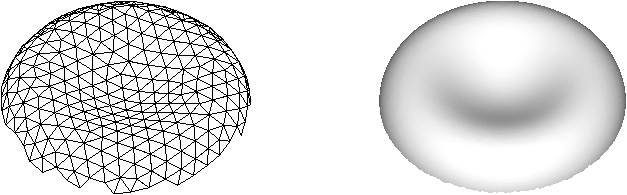
\includegraphics[width=25em]{network2continuum.pdf}};
\node[text width=10em] at (-3,2.2) {\bf 弹簧常数, 弯曲常数, 体积约束, 面积约束};
\node[text width=10em] at ( 3,2.2) {\bf 剪切模量, 压缩模量, 杨氏模量, 弯曲刚度};
\node[text width=5em] at (-2.8,-1.8) {\bf 粒子模型};
\node[text width=5em] at ( 2.8,-1.8) {\bf 连续模型};
\draw[very thick, <->, >=stealth'] (-1,2.2) -- (1, 2.2);
\draw[very thick, <->, >=stealth'] (-0.8,0) -- (0.8, 0);
\draw[very thick, <->, >=stealth'] (-1.2,-2.2) -- (1.2, -2.2);
\end{tikzpicture}

\caption{\label{fig:network2continuum} 粒子模型(节点为粒子)和连续模型的示意图}
\end{figure}
\end{frame}

\begin{frame}
\frametitle{红细胞的运动与变形模拟: 应力分析与推导}
\note{\textcolor{red}{375-390s}}
\note[item]{为了匹配这些参数, 要对珠簧链构成的网络单元进行力学分析, 通过对图10的六边形单元应力分析, 可以得到剪切模量与弹簧常数的关系}
\begin{columns}
\begin{column}[c]{0.5\textwidth}
\begin{figure}[!htb]
\centering
\begin{tikzpicture}[
    scale = 0.7,
    axis/.style={very thick, ->, >=stealth'},
    important line/.style={thick},
    dashed line/.style={dashed},
    pile/.style={thick, ->, >=stealth', shorten <=2pt, shorten
    >=2pt},
    every node/.style={color=black}]
    % axis
    \filldraw[fill=gray!10,draw=gray!10] (15:3) -- 
         (75:3) -- (135:3) -- (195:3) -- (255:3) -- (315:3) -- (375:3);
    \filldraw[fill=gray!30,draw=gray!30] (45:1.732)  -- (105:1.732) -- (165:1.732) -- (225:1.732) -- (285:1.732) -- (345:1.732) -- (405:1.732);
    \draw[axis] (0,0)  -- (4.1,0) node(xline)[right]{$x$};
    \draw[axis] (0,0)  -- (0,3.8) node(yline)[above]{$y$};
    \draw[thick] ( 15:-3) --node[very near end, below]{$a$} ( 15:3) node[right]{$(a_x, a_y)$};
    \draw[thick] ( 75:-3) --node[very near end, right]{$b$} ( 75:3) node[right]{$(b_x, b_y)$};
    \draw[thick] (135:-3) -- (135:3) node[above]{$(c_x, c_y)$};
    \draw[thick] (15:3) -- node[right] {\,$c=|\vec{b}-\vec{a}|$}
         (75:3) -- (135:3) -- (195:3) -- (255:3) -- (315:3) -- (375:3);
    \draw[thick] (45:2.2) node{$\mathbf{A}$} (105:1) node{$\mathbf{S}$} (170:0.4) node{$v$};
    \fill (0,0) circle (2.5pt);
    \draw[densely dashed,thick] (45:1.732)  -- (105:1.732) -- (165:1.732) -- (225:1.732) -- (285:1.732) -- (345:1.732) -- (405:1.732);
\end{tikzpicture}


\caption{\label{fig:network2continuum} 六边形单元}
\end{figure}
\end{column}
\begin{column}[c]{0.5\textwidth}
在$V$周围$2A$面积上的应力
\[
\tau_{\alpha\beta} = -\frac{1}{2A}\sum_{\chi=\{a,b,c\}} \frac{f(\chi)}{\chi}\chi_\alpha \chi_\beta
\]
剪切模量由$\mu_0=\frac{\partial \tau_{xy}}{\partial \gamma}|_{\gamma=0}$得到.
\[
\mu_0 = -\frac{A_0}{l_0}\frac{\partial \frac{f(r)}{r}}{\partial r}\bigg|_{r=l_0}-\frac{3f(l_0)l_0}{4A_0}
\]

\end{column}
\end{columns}
\end{frame}

\begin{frame}
\frametitle{红细胞的运动与变形模拟: 弯曲能分析与推导}
\note{\textcolor{red}{390-405s}}
\note[item]{类似的, 对由珠簧链构成的相邻两三角形单元进行分析, 把连续模型中的弯曲能量与粒子方法中的弯曲能量相匹配, 可以得到弯曲常数与弯曲刚度间的联系.}
\begin{columns}
\begin{column}[c]{0.5\textwidth}
\begin{figure}[!htb]
\centering
\begin{tikzpicture}[scale = 0.7,rotate around = {15:(0,0,0)},
    axis/.style={very thick, ->, >=stealth'},
    important line/.style={thick},
    dashed line/.style={dashed, thin},
    pile/.style={thick, ->, >=stealth', shorten <=2pt, shorten
    >=2pt},
    every node/.style={color=black}]
    \coordinate (O) at (0,0);
    \coordinate (A) at (4.12,4.64);
    \coordinate (B) at (4.84,1.8);
    \coordinate (C) at (6.48,4.08);
    \coordinate (D) at (7.6,2.0);
    \coordinate (e) at (33.89:6.31);
    \coordinate (f) at (22.67:6.85);
    \coordinate (X) at ($ (B)!.625!(C) $);

    \filldraw[fill=gray!20,draw=gray!20,opacity=0.2] (O) -- (A) -- (C) -- cycle;
    \filldraw[ball color= gray!20,draw=gray!80,opacity=0.2] (O) -- (D) -- (C) -- cycle;
    \filldraw[fill=gray,draw=gray,opacity=0.2] (O) -- (B) -- (C) -- cycle;
    \draw [thick, gray] (O) -- (C) (O)-- node[near end,below]{$S$}(X); 

    \draw [very thick, dashed, black!80] (O) -- (e) (O) -- (f);
    \filldraw[fill=gray!10,draw=gray!10,opacity=0.5] (A) -- (C) -- (B) -- cycle;
    \filldraw[ball color= gray!20,draw=gray!80,opacity=0.5] (D) -- (C) -- (B) -- cycle;

    \draw[thick] (A) -- node[above] {a} (C) -- (B) -- cycle;
    
    \draw[thick] (C)-- (D) -- (B); 
    \draw[thick] (O) -- node[above]{$R$} (A) 
          (O) -- (B) 
          (O) -- node[below]{$R$} (D);
\draw[thick] (e) -- node[near start,below] {$r$} (X) (f) --  node[near start, above] {$r$} (X);
    \draw[black!80] ($ (X)!.15!(C) $) -- ($ (X)!.15!(C)!0.08!-80:(B) $) -- ($ (X)!.2!(e) $)
($ (X)!-.15!(C) $) -- ($ (X)!-.15!(C)!0.08!80:(B) $) -- ($ (X)!.19!(f) $);
    \draw [axis] (e) -- (33.89:9) node[left] {$\mathbf{n}_1$};
    \draw [axis] (f) -- (22.67:8.8) node[above] {$\mathbf{n}_2$};
    \draw (22.67:8.2)  arc(22.67:33.89:8.2) (28:8.5) node{$\theta$};
    \fill (O)    node[left]{$O$}    circle (2.5pt) 
          (33.89:6.31) circle (2pt) 
          (22.67:6.85) circle (2pt);
    \filldraw[fill=gray!20,draw=black,opacity=0.5] (O) -- (A) -- (B) -- cycle;
    \filldraw[ball color= gray!20,draw=black,opacity=0.2] (O) -- (D) -- (B) -- cycle;
\end{tikzpicture}

\vspace{-2em}
\caption{\label{fig:network2continuum} 三角形单元}
\end{figure}
\end{column}
\begin{column}[c]{0.5\textwidth}
由Helfrich模型得到弹性模弯曲的能量
\[
E_c= 8\pi k_c(1-R/R_0)^2+4\pi k_g
\]
网状模型中膜弯曲的势能
\[
V_{\text{bending}}=\sum_{j\in1\cdots N_s}k_b[1-\cos(\theta_j-\theta_0)]
\]
由$E_c=V_{\text{bending}}$, 且$k_g=-4k_c/3$得
$k_b=2k_c/\sqrt{3}$.
\end{column}
\end{columns}
\end{frame}


\begin{frame}
\frametitle{红细胞的运动与变形模拟: 剪切流与泊肃叶流(2D)}
\note{\textcolor{red}{405-420s}}
\note{在选择了适当的参数后, 我们首先对二维红细胞在剪切流与泊肃叶流(2D)作了模拟, 模拟到得的形态与实验和文献的结果吻合}
\begin{columns}
\begin{column}[c]{0.5\textwidth}
\begin{figure}
\centering
\animategraphics[width=\textwidth, poster=first, autoplay, every = 3]{5}{./animate/shear2d/}{0}{58}
\caption{剪切流中红细胞(2D)的运动与变形}
\end{figure}
\end{column}
\begin{column}[c]{0.5\textwidth}
\begin{figure}
\centering
\animategraphics[width=\textwidth, poster=first, autoplay, every = 2]{5}{./animate/poise2d/}{0}{43}
\caption{泊肃叶流中红细胞(2D)的运动与变形}
\end{figure}
\end{column}
\end{columns}
\end{frame}




\begin{frame}
\frametitle{红细胞的运动与变形模拟: 三维红细胞拉伸}
\note{\textcolor{red}{420-440s}}
\note[item]{其次, 我们对三维红细胞的拉伸实验做了模拟}
\note[item]{图14中是红细胞在不同拉力下的直径变化, 黑色是实验结果, 蓝点和红点是我们计算结果. 可以看出计算结果与实验结果吻合良好.}
\begin{columns}
\begin{column}[c]{0.4\textwidth}
\begin{center}
\animategraphics[width=0.78\textwidth, poster=first, autoplay, loop]{5}{./animate/RBC/90-0/}{1}{50}\\
\animategraphics[width=\textwidth, poster=first, autoplay, loop]{5}{./animate/RBC/30/}{1}{50}
\end{center}
\end{column}
\begin{column}[c]{0.6\textwidth}
\begin{figure}[!htb]
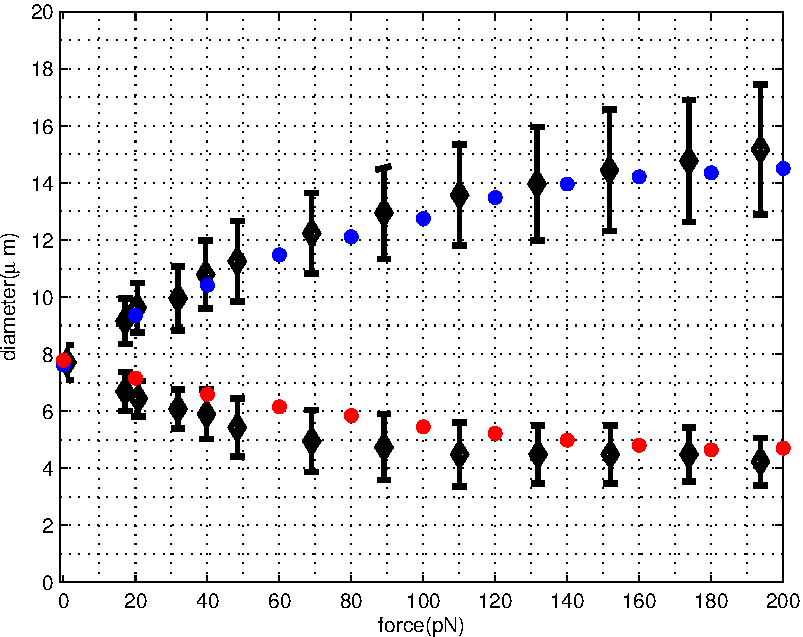
\includegraphics[width=\textwidth]{lp.pdf}
\caption{红细胞在不同拉力下的直径变化}
\end{figure}
\end{column}
\end{columns}
\end{frame}

\begin{frame}
\frametitle{癌细胞吸入实验的模拟}
\note{\textcolor{red}{440-460s}}
\note[item]{在成功模拟红细胞的基础上, 我们参考红细胞的模型, 又对乳腺癌细胞进行建模,并对乳腺癌细胞吸入实验进行了模拟}
\animategraphics[width=\textwidth, poster=first, autoplay, every=3]{5}{./animate/cell3d/}{1}{109}
\end{frame}

%\frame{\frametitle{癌细胞的模拟: 细胞构型}
%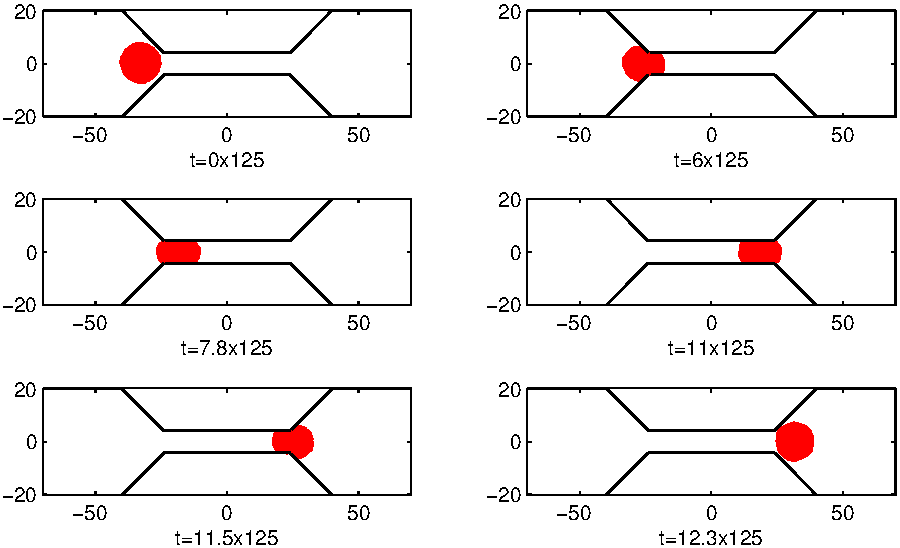
\includegraphics[width=1\textwidth]{cell.pdf}
%}

%\frame{\frametitle{癌细胞的模拟: 位移与速度}
% \begin{columns}
%  \begin{column}[b]{0.5\textwidth}
%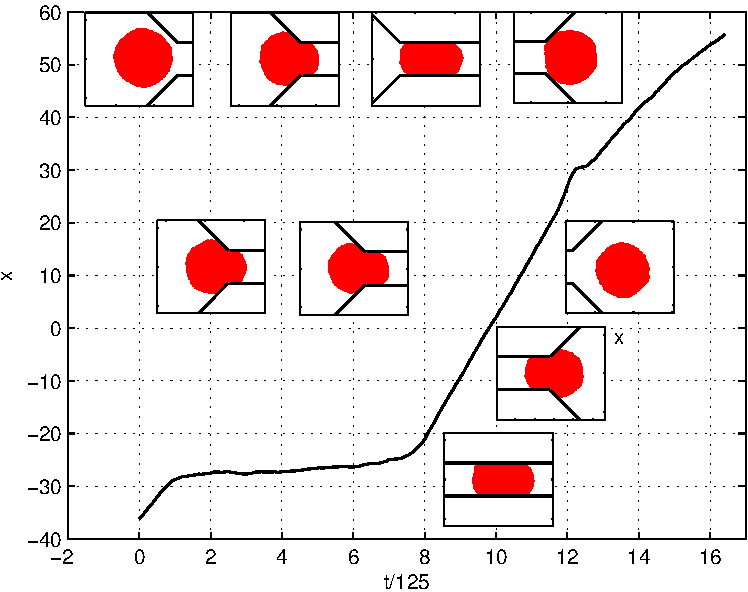
\includegraphics[width=1\textwidth]{x.pdf}
%  \end{column}
%  \begin{column}[b]{0.5\textwidth}
%\begin{center}
%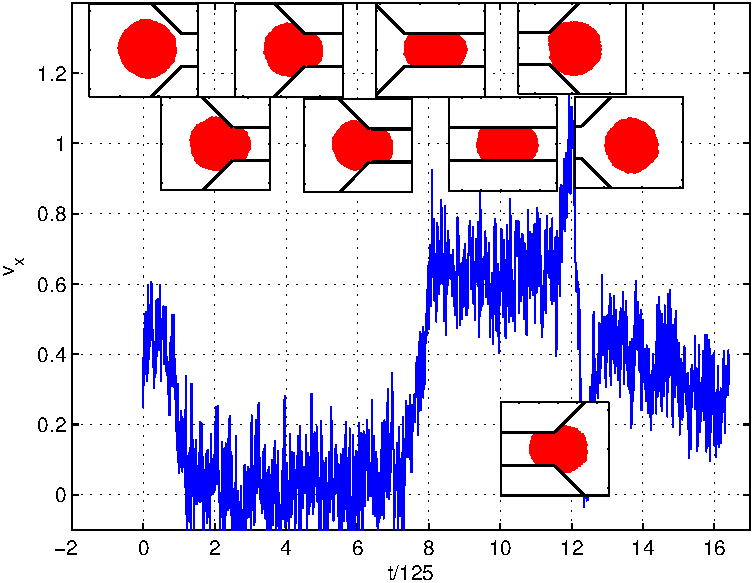
\includegraphics[width=1\textwidth]{cellLenght.pdf}
%\end{center}
%  \end{column}
%\end{columns}
%}

\frame{\frametitle{癌细胞吸入实验的模拟: 构型与实验对比}
\note{\textcolor{red}{460-475s}}
\note[item]{左图为实验得到的细胞构型结果, 右图为我们计算得到的结果, 结果显示计算得到的细胞构型与实验吻合较好}
 \begin{columns}
  \begin{column}[b]{0.5\textwidth}
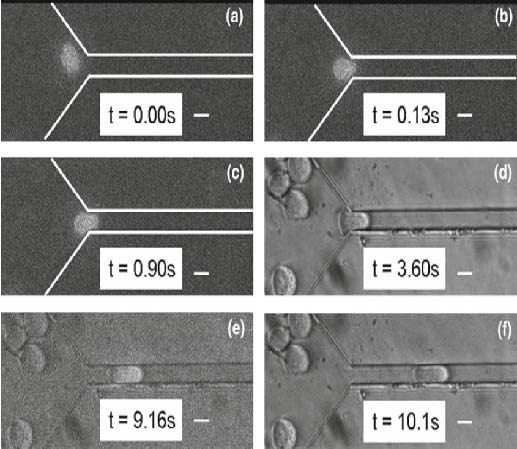
\includegraphics[width=\textwidth]{cell.jpg}
  \end{column}
  \begin{column}[b]{0.5\textwidth}
\begin{center}
\fbox{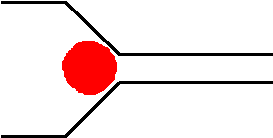
\includegraphics[width=0.43\textwidth]{cellconfig01.pdf}}
\fbox{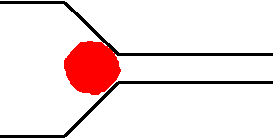
\includegraphics[width=0.43\textwidth]{cellconfig02.pdf}}

\vspace{5pt}

\fbox{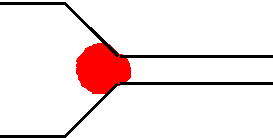
\includegraphics[width=0.43\textwidth]{cellconfig03.pdf}}
\fbox{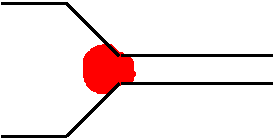
\includegraphics[width=0.43\textwidth]{cellconfig04.pdf}}

\vspace{5pt}

\fbox{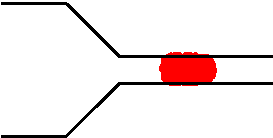
\includegraphics[width=0.43\textwidth]{cellconfig05.pdf}}
\fbox{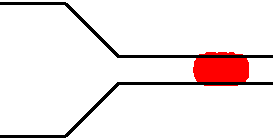
\includegraphics[width=0.43\textwidth]{cellconfig06.pdf}}

\vspace{1pt}
%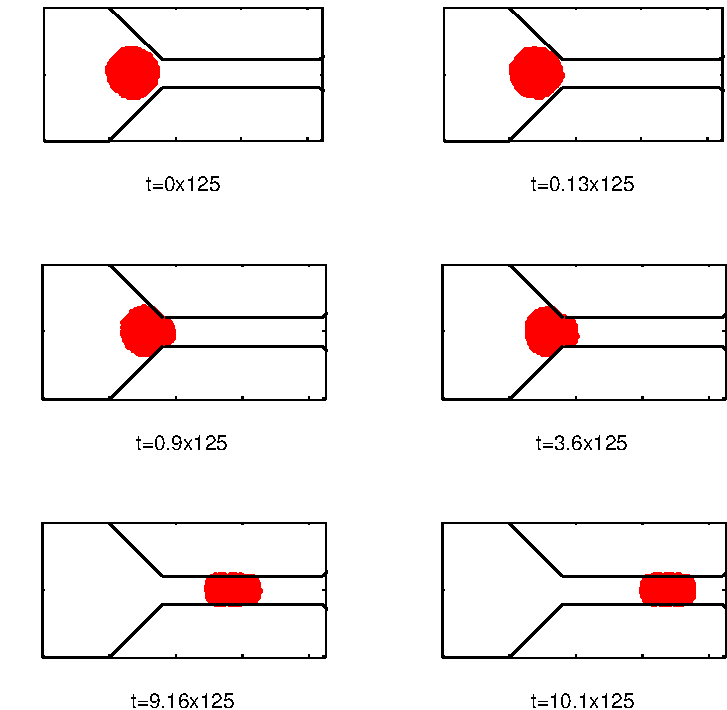
\includegraphics[width=0.98\textwidth]{cellconfig.pdf}
\end{center}
  \end{column}
\end{columns}
}

%\frame{\frametitle{癌细胞的模拟: 速度与实验对比}
% \begin{columns}
%  \begin{column}[b]{0.46\textwidth}
%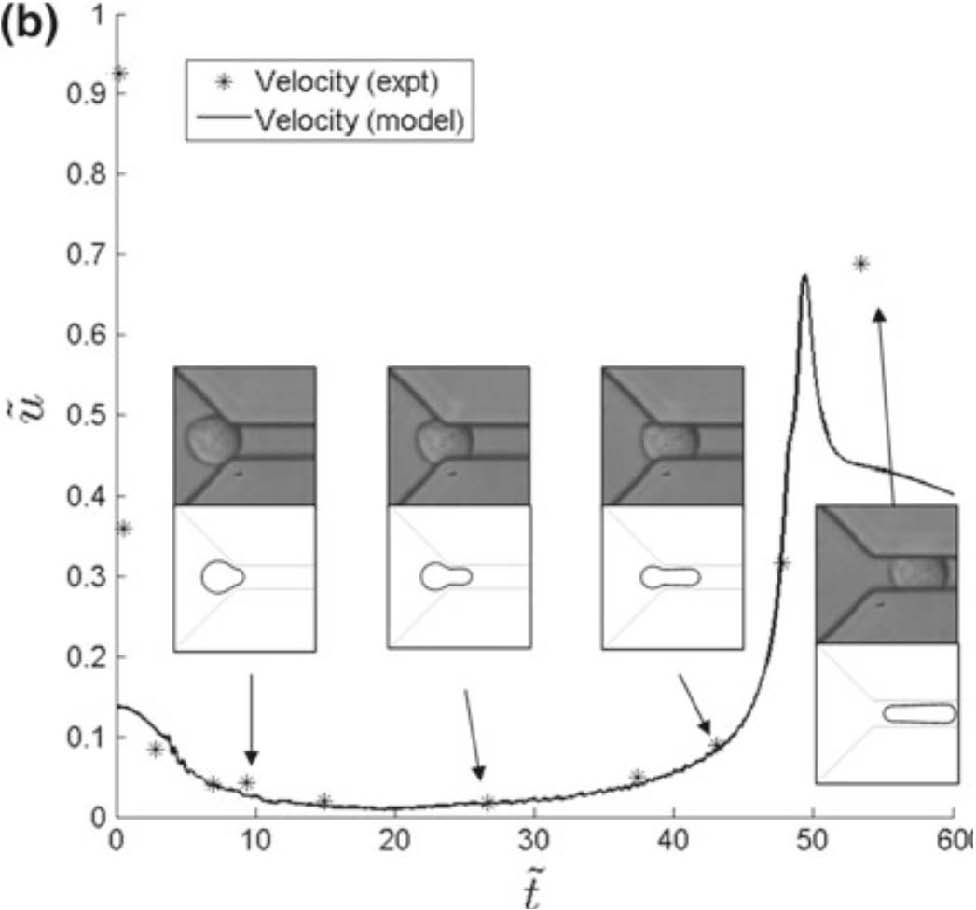
\includegraphics[width=1\textwidth]{vx.jpg}
%  \end{column}
%  \begin{column}[b]{0.54\textwidth}
%\begin{center}
%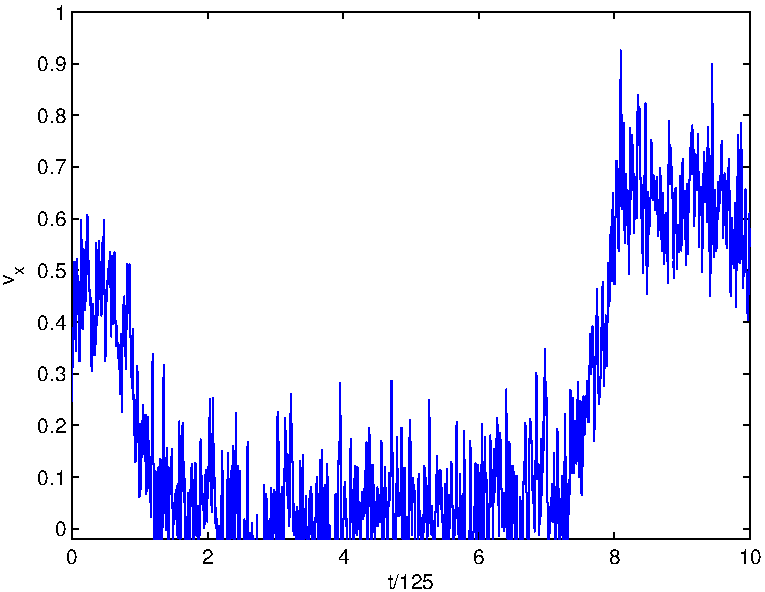
\includegraphics[width=1\textwidth]{cellvx.pdf}
%\end{center}
%  \end{column}
%\end{columns}
%}

\begin{frame}
\frametitle{血红细胞与癌细胞的DPD模拟: 小结}
\note{\textcolor{red}{475-495s}}
\note[item]{我们还比较了细胞的运动速度等结果, 得到了一些定性和半定量的结果.}
\begin{itemize}
\item 应用DPD方法对红细胞做了初步模拟, 二维剪切流与泊肃叶流及拉伸情况与实验观察或其他文献报告吻合, 验证了模型和程序的合理性.
\item 采用类似的方法, 对乳腺癌细胞的吸入实验展开了初步模拟. 模拟所得结果与实验基本吻合.
\item 乳腺癌细胞在开始进入微缩通道时减速, 拉长自身, 当细胞绝大部进入微缩结构后, 迅速加速直至细胞完全进入微缩通道; 细胞在微缩通道中的运动速度几乎不变. 当细胞从微缩结构的出口离开时, 又逐渐恢复了球形.  数值模拟所得到的细胞变形, 吸入及释放复原的形态与实验结果吻合.
\item 通过进一步定量分析, 有望对红细胞和乳腺癌细胞开展更深入研究.
\end{itemize}
\end{frame}


\section{研究计划}
\note{\textcolor{red}{495-555s}}
\begin{frame}
\frametitle{研究计划}
\note{下面看一下我的研究计划, 淡蓝色的模块是已经或正在做的工作, 淡红色是还没有做的工作}
\note[item]{下一部我们打算先完细胞这块的工作}
\note[item]{然后把高分子推广到多物理场情况下}
\note[item]{再对方法做工作, 对势函数进行一些改进, 对MD,DPD,SPH的藕合作一些尝试}
\note[item]{最后结合高性能计算, 实现一些大规的模拟}

\tikzstyle{decision} = [diamond,aspect=2, draw,fill=blue!20, 
    text width=32, text badly centered, inner sep=0pt]
\tikzstyle{block} = [rectangle, draw, fill=blue!20, 
    text width=43, text centered, rounded corners, minimum height=25]
\tikzstyle{line} = [draw, -latex', very thick]
\tikzstyle{cloud} = [draw, ellipse,fill=red!20, node distance=75,
    text width=28, minimum height=0]
{\footnotesize
\begin{tikzpicture}[scale=0.76]
    % Place nodes
    \node [block](A) at (0,-1) {\bf 研究内容};
    \node [block](B) at (3,-1) {\bf 应用};
    \node [block](C) at (3,3.5) {\bf 方法};
    \node [block](D) at (3,-4.5) {\bf 并行 CPU/GPU};

    \node [block](E) at (6,0.0) {高分子};
    \node [block](F) at (6,-2.0) {红细胞};
    \node [block, fill=red!30](G) at (6,3.5) {\textcolor{blue}{MD, DPD, SPH藕合}};
    %\node [block](H) at (6,-3.5) {CPU};

    \node [block, fill=red!30](I) at (6,1.5) {\textcolor{blue}{多物理场}};
    \node [block, fill=blue!20](J) at (6,-3.5) {\textcolor{blue}{乳腺癌细胞}};
    %\node [block](K) at (9,-3.5) {\textcolor{blue}{GPU}};

    \node [block, fill=red!30](L) at (12,-1) {\textcolor{blue}{高性能大规模计算}};

    \node [block, fill=red!30](M) at (3,1.5) {\textcolor{blue}{势函数}};
    \node [decision](N) at (9.5,-1) {\scriptsize 珠簧链};
    \node [decision](O) at (3,-2.8) {\scriptsize 简单流体};

    \path [line] (A) -- (B);
    \path [line] (A) |- (C);
    \path [line] (A) |- (D);
    \path [line] (B) -| (E);
    \path [line] (B) -| (F);
    \path [blue, line, dashed] (C) -- (G);

    \path [line] (E) -- (I);
    \path [line] (F) -- (J);

    \path [blue, line, dashed] (D) --(12.5,-4.5)-- (12.5,-1.6);
    \path [blue, line, dashed] (G) --(12.5,3.5)-- (12.5,-0.4);
    \path [blue, line, dashed] (G) -- (6,2.5) -- (4.5,2.5)-- (4.5, 0.25) -- (3, 0.25);
    \path [blue, line, dashed] (L) |- (I);
    \path [blue, line, dashed] (L) |- (J);
    \path [blue, line, dashed] (L) |- (E);
    \path [blue, line, dashed] (L) |- (F);

    \path [blue, line, dashed] (C) -- (M);
    \path [blue, line, dashed] (M) -- (B);
    
    \path [line] (E)--node[sloped, fill=red!8.5]{\tiny 验证} (N);
    \path [line] (N)--node[sloped, fill=red!8.5]{\tiny 应用} (F);
    \path [line] (O)--node[left]{\tiny 验证} (B);

\end{tikzpicture}}

\end{frame}


%\includepart{thebibliography}

%%%%%%%%%%%%%%%%%%%%%%%%%%%%%%%%%%%%%%%%%%%%%%%%%%%%%%%%%%%%%%%%%%%%%%%%%%
%%
%% ������һ����ʾThank you!!!�����Ķ���
%%

\newcount\opaqueness
\plainframe{
  \itshape
  \Large
    \begin{centering}
      \Huge Thank You!!!\par
    \end{centering}
} 

\end{document}
